\chapter{Эмоциональные состояния на уровне нейробиологических процессов.}
\label{chap:theoretical_development}

Исследование эмоциональных вычислений как поиск моделей, объясняющих эмоции, начиналось в областях психологии, нейропсихологии и философии. Эволюционная теория происхождения эмоций Ч. Дарвина объясняла эмоции как приспособительные механизмы, жизненно важные для адаптации организма к условиям жизни. Д. Пейпец выдвигал гипотезу о единой системе, объединяющей структуры мозга, участвующие в формировании эмоций, — позже она получила название лимбической системы. Исследования Ф. Барда, подкрепленные данными физиологии, свидетельствовали, что физиологические проявления и субъективные переживания эмоциональных процессов происходят одновременно, благодаря расщеплению возбуждающего нервного импульса в таламусе. Двухфакторная теория эмоций С. Шехтера разделяла эмоцию на эти же два компонента: физиологическое возбуждение и его когнитивную интерпретацию.


Десятилетиями нейробиологи публиковали результаты экспериментов о том, нейроны какого типа и в какой части мозга проявляют активность, в зависимости от состояния организма, в том числе и эмоционального состояния. Эти многочисленные данные собраны и обобщены доктором психиатрии Хьюго Левхеймом, который предложил на их основе новую трёхмерную модель эмоций.\cite{lovheim2012} Базовые эмоции (аффекты), объясняемые в его работе нейробиологически, берутся из психологической модели Сильвана Томкинса.\cite{tomkins1962, tomkins1963, tomkins1991} Теория аффектов Томкинса разделяет 9 «первичных» эмоций (наблюдаемых с рождения) на категории и соединяет каждую с типичным физиологическим проявлением, позой, выражением лица. Например, злость — покрасневшее лицо, сжатые челюсти, сдвинутые брови. Из этих 9 эмоций Левхейм не стал вводить в модель эмоцию реакции на неприятный запах, остальные 8 включены и присутствуют на рисунке ~\ref{fig:cube_0}.


\begin{figure}
	\centering
	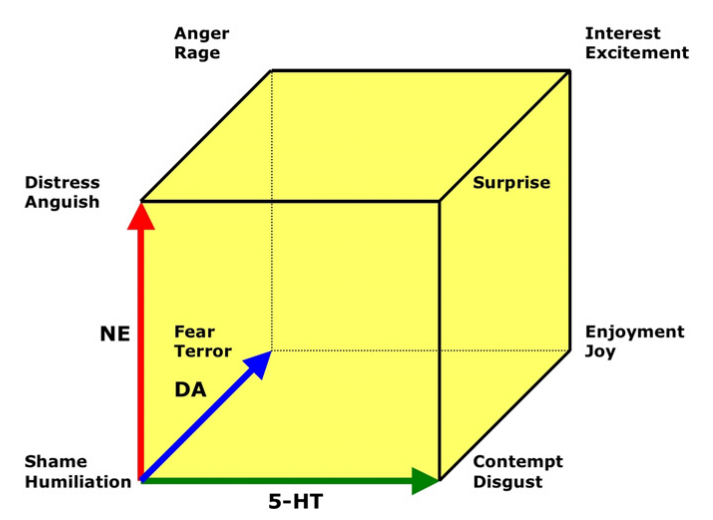
\includegraphics[width=\linewidth]{cube_0}
	\caption{Модель Левхейма, задающая трёхмерное пространство эмоций через нейромодуляторы серотонин, дофамин и норадреналин.\cite{lovheim2012}}
	\label{fig:cube_0}
\end{figure}


Тремя измерениями модели Левхейма являются уровни концентрации моноаминовых нейромодуляторов серотонин, дофамин и норадреналин — минимально необходимое количество для того, чтобы специально упрощённая модель оставалась реалистичной. Нейромодуляторы это биологически активные химические вещества,  контролирующие процессы, происходящие между нейронами. Системы названных моноаминовых нейромодуляторов эволюционно сохраняются в различных организмах, они контролируют поведение как людей, так и крыс, лобстеров, пустынной саранчи и др. Эти системы обеспечивают гибкость поведения и способность адаптироваться к постоянно изменяющейся окружающей среде, сами по себе также являются динамичными.\cite{Benarroch17112009}


Нейронная активность может модифицироваться и перенастраиваться, когда концентрация нейромодулятора повышается из-за активности конкретных зон мозга (например, голубоватого пятна, в случае норадреналина). Нейромодулятор разносится по другим областям мозга, где влияет на многочисленные рецепторы подходящего типа. Это может усиливать или ослаблять связь между нейронами, если связь также была активна совсем недавно (эффект собаки Павлова), менять свойства нейронов.\cite{parsingreward} У таких нейромодулирующих систем существуют анатомические привилегии широкого доступа к многим областям нервной системы, и они идеально расположены для регулирования всех процессов обработки и хранения информации в мозге. Нейромодулирующие системы принимают активное участие в работе двигательных, чувственных и когнитивных функций.\cite{zarrindast} Их роль в работе мозга настолько велика, что, несмотря на внушительное количество уже имеющихся экспериментальных данных, вопросы взаимодействия нейромодуляторов друг с другом, точного механизма их функционирования и прочие остаются открытыми, требующими длительного дальнейшего изучения.


На рисунке 1 зелёная ось «5-HT» обозначает уровень концентрации нейромодулятора серотонин. В человеческом организме серотонин отвечает за регуляцию поведения, аппетит, обучение, общение — за всё, что делают в спокойном состоянии. Низкий уровень серотонина влечёт сонливость, высокий уровень серотонина повлечёт за собой половое влечение,  быстрое переваривание пищи, чувство эйфории и ощущение непобедимости. Серотонин влияет на уверенность в себе, особенно после верно принятых решений, и участвует в контроле агрессии. В точке, где концентрация серотонина максимальна, а остальных минимальна, расположена эмоция сытости/отвращения/презрения.


Красная ось «NE» - уровень концентрации нейромодулятора норадреналин, или норэпинефрин. Уровень его концентрации повышается в ответ на стрессовые ситуации, раздражители и на всё новое, либо неожиданное. Высокий уровень норадреналина вызывает повышение бдительности и скорости реакции, концентрацию внимания, улучшение обработки сенсорных входов, повышение уровня возбуждения. В точке, где концентрация норадреналина максимальна, а остальных минимальна, расположена эмоция страдания/отчаяния. Млекопитающее испытывает ощущение бедствия, когда произошло что-то непоправимое или болезненное, и максимально сконцентрировано на этом событии.


Синяя ось «DA» - уровень концентрации нейромодулятора дофамин. Он отвечает за наслаждение и удовольствие от выполненного дела, вкусной еды, приятных ощущений, даёт ощущение награды, таким образом закрепляя важные для выживания и благосостояния действия. Дофамин используется мозгом для оценки действий и мотивации, а также для активации моторных функций. В точке, где его концентрация максимальна, а остальных минимальна, находится эмоция «страх».


В точке, где концентрация каждого нейромодулятора минимальна, располагается эмоция «стыд», когда нет ни сфокусированности внимания, ни чувства удовлетворения, ни уверенности в себе. Повышенные уровни дофамина и норадреналина влекут «ярость», серотонина и норадреналина - «удивление», дофамина и серотонина — спокойное «удовольствие». Высокий уровень концентрации всех трёх нейромодуляторов в модели Левхейма связан с эмоцией активной «заинтересованности», «увлеченности».


Отображение клеточных реакций на вычислительный процесс должно быть осуществлено так, чтобы при удалении всей биохимии, отсутствии настоящих моноаминов и белков удалось сохранить роли нейромодуляторов в системе. Были предложены следующие аналогии \cite{talanov2014}, зафиксированные на рисунке ~\ref{fig:cube_1}:
\begin{description}
\item[Использование вычислительных ресурсов] подвержено влиянию дофамина и серотонина, которые усиливают спайковую активность нейронов в системе и поэтому увеличивают занятость "искусственного мозга" вычислительной системы.
\item[Распределение вычислений] регулируется норадреналином. Чем выше уровень норадреналина, тем больше вычислительной мощности будет сконцентрировано на действии. Это соответствует переключению внимания в мозге живого существа.
\item[Распределение оперативной памяти] регулируется норадреналином. Это соответствует перераспределению мыслительных процессов, чтобы полностью сосредоточиться на источнике опасности, боли или неожиданном событии. 
\item[Объём внешней памяти] испытывает воздействие серотонина и дофамина. Например, более высокие концентрации обоих нейромодуляторов сделают систему более эффективной при запоминании внешнего стимула. Сильные эмоции создают более полные и глубокие воспоминания, состоящие из большего количества данных, чем обычное воспоминание.
\item[Связность] испытывает влияние серотонина. Более высокая концентрация этого нейромодулятора увеличивает количество связей между ячейками памяти, воспоминания связываются одно с другим.
\end{description}



\begin{figure}
	\centering
	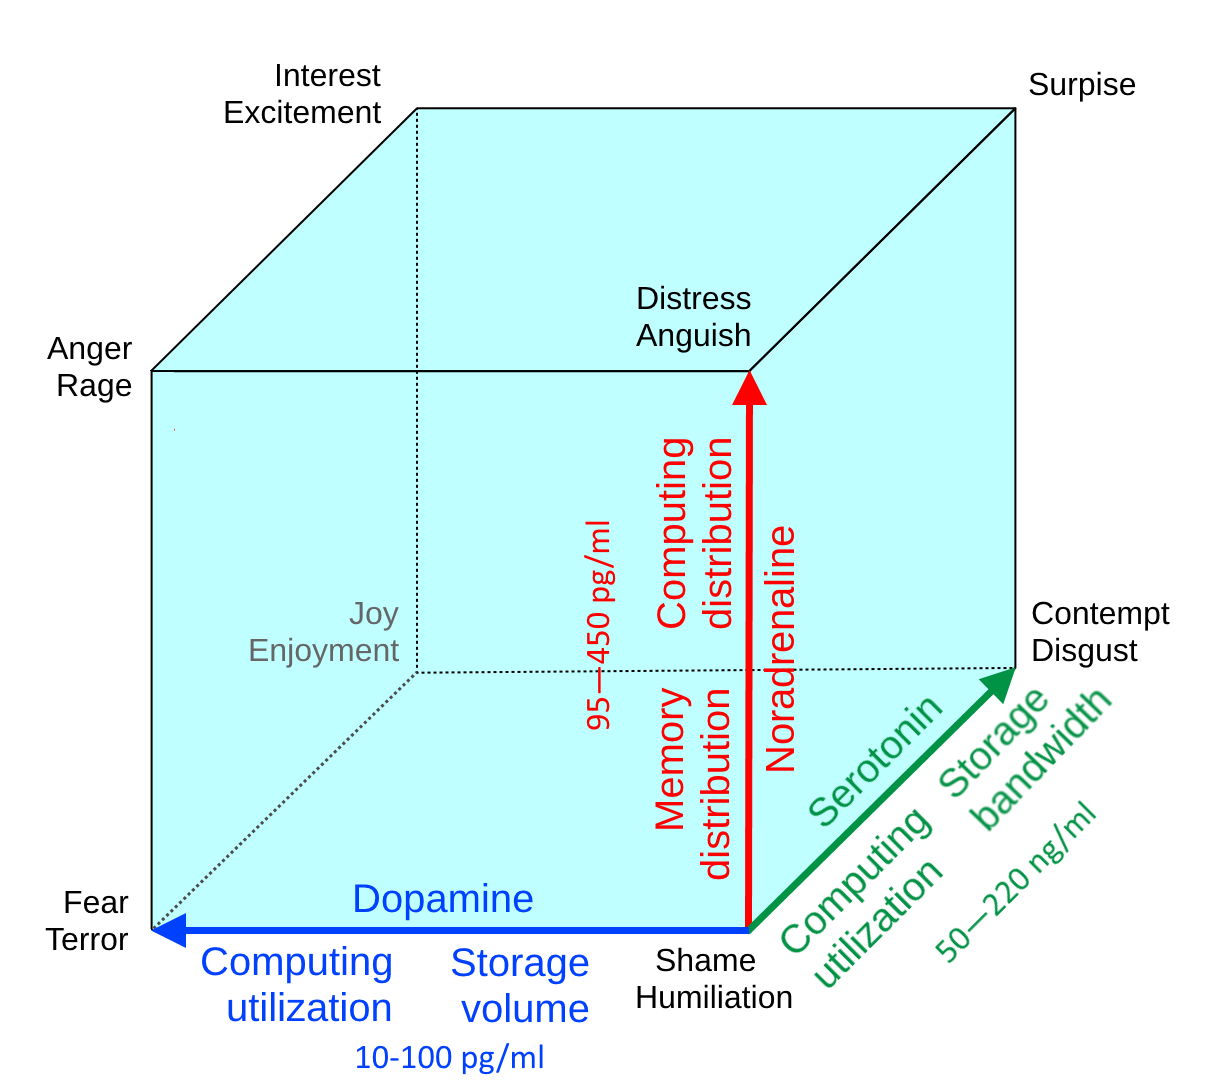
\includegraphics[width=\linewidth]{cube_1}
	\caption{Дополненная модель Левхейма. Проведение аналогии роли нейромодуляторов с вычислительными процессами. Норадреналин (красный) влияет на распределение вычислений и оперативной памяти. Серотонин (синий) увеличивает объём внешней памяти, использование вычислительных ресурсов и связность. Дофамин (зелёный) регулирует использование вычислительных ресурсов и объём внешней памяти.}
	\label{fig:cube_1}
\end{figure}
